\section{Replacing a site by a mesoscopic square}
\label{sec:sewing}

The expansion in the preceding section reduces the problem to identifying
signed kernels at finitely many separated insertion points.  A microscopic
insertion is not itself a continuous critical observable.  We compare it
with forcing the colors in a square of fixed positive size, which is covered
by Proposition~\ref{prop:critical-tests}.  Approximating microscopic pivotal
behavior by mesoscopic crossing data is central to the construction of
Garban, Pete, and Schramm~\cite[Section~4]{garbanpete-schramm-pivotal}.
Here the comparison must preserve the signs of history weights and allow
two color replicas on the same Poisson geometry.  This section proves that comparison before taking any
limit of microscopic pivotal amplitudes.

\subsection{Mixed kernels and the comparison statement}

Fix a finite family of polygonal quads, a bounded function $F$ of their
crossing indicators at finitely many labeled times, and either one or two
color replicas.  Assume $|F|\leq 1$.  Fix $k\geq1$ insertion points
$\boldsymbol x=(x_1,\ldots,x_k)$ in a compact set of configurations on which
the points are mutually separated and stay a positive distance from all
quad boundaries and from the boundary of the integration box.  There is
one active replica label at each insertion point, and a signed measure
$w_i$ of total mass zero on that replica's finite history space.  Its total
variation is bounded by a fixed constant.  Repeated labels at a single
site were disposed of in Proposition~\ref{prop:expansion-bound}.

A \emph{site insertion}, denoted $s$, has the meaning used in the expansion:
in the Poisson model add a nucleus at $x_i$ and impose the selected history
on its cell; on the triangular lattice impose it at the site $x_i$.
A \emph{square insertion}, denoted $d$, uses the ordinary geometry, without
adding a Poisson nucleus, and imposes the selected history on every cell
meeting
\[
 B_\infty(x_i,h)=x_i+[-h,h]^2.
\]
Write
\[
 K_e^{\boldsymbol t}(F;\boldsymbol x,\boldsymbol w),
 \qquad \boldsymbol t\in\{s,d\}^k,
\]
for the resulting signed kernel, with the replica labels suppressed.
All unspecified colors are fair and constant across the tested times.
If two instructions apply to one cell, use the instruction with the smaller
insertion index.  Localization shows that such conflicts between separated
insertion regions have exponentially small probability for fixed $h$ and
small $e$.  The same convention applies to forced-square critical tests.
We remove the large-box truncation in these fixed-degree kernels; its
exponentially small error remains negligible after their normalizations.

Set
\[
 a_e=A_e(b_e,1),\qquad a_{e,h}=A_e(h,1),\qquad
 \gamma_e(s)=a_e,\quad \gamma_e(d)=a_{e,h}.
\]
Independent localized probes around the insertion points, using
Lemma~\ref{lem:localization}, give
\begin{equation}
 \bigl|K_e^{\boldsymbol t}(F;\boldsymbol x,\boldsymbol w)\bigr|
 \leq C\prod_{i=1}^k \gamma_e(t_i).
 \label{eq:mixed-kernel-upper}
\end{equation}
Indeed, the centered integral vanishes unless changing each inserted
history can affect one of the tested crossings, for some settings of the
other histories.  Outside its insertion region this implies four
alternating arms on the unchanged fair bits.  The probes start at a
constant multiple of $b_e$ or $h$ and end at a fixed radius smaller than
the separation distances.  Cells extending out of an insertion region
are handled by the outermost failed occupancy test, rather than by assuming
that their diameters are bounded.  Quasi-multiplicativity compares the
probe costs to $a_e$ and $a_{e,h}$.  Constants may depend on the fixed
compact set and the bounds on the weights, but not on $e$ or sufficiently
small $h$.

Let $G_x=\mathbf1_{C_{x+Q_0}}$, where
$Q_0=[-1,1]\times[-1/2,1/2]$ has its vertical sides as target arcs.
Use one replica and the one-time weight
$\Delta=\delta_1-\delta_0$ at $x$.  Denote the corresponding site and
square kernels by
\[
 S_e=K_e^s(G_x;x,\Delta),\qquad
 D_e(h)=K_e^d(G_x;x,\Delta).
\]
Stationarity makes these independent of $x$; triangular centers are lattice
sites.  Monotonicity and \eqref{eq:mixed-kernel-upper} give
$0\leq S_e\leq C a_e$ and $0\leq D_e(h)\leq C a_{e,h}$.

\begin{lemma}[A square can transmit a pivotal change]
\label{lem:disk-lower}
There is $c>0$ such that, for every sufficiently small fixed $h>0$ and all
sufficiently small $e$ depending on $h$,
\begin{equation}
 D_e(h)\geq c a_{e,h}.
 \label{eq:disk-lower}
\end{equation}
The same assertion holds for the one-time square-insertion kernel of a
fixed square or rectangle crossing when its center varies in a sufficiently
small open neighborhood of the center of that test.  The constant is
uniform over that neighborhood.
\end{lemma}

The proof is given below, after the needed arm-extension construction.
Our principal assertion compares products, so that no microscopic
amplitude has to be known in advance.

\begin{proposition}[Signed relative replacement]
\label{prop:replacement}
Under the preceding assumptions, fix the types $t_2,\ldots,t_k$ and put
\[
 K_s=K_e^{(s,t_2,\ldots,t_k)}(F;\boldsymbol x,\boldsymbol w),\qquad
 K_d=K_e^{(d,t_2,\ldots,t_k)}(F;\boldsymbol x,\boldsymbol w),\qquad
 P_e=\prod_{i=2}^k \gamma_e(t_i).
\]
The empty product is $1$.  In either model,
\begin{equation}
 \lim_{h\downarrow0}\limsup_{e\downarrow0}
 \sup_{\boldsymbol x}
 \frac{|K_sD_e(h)-K_dS_e|}{P_e a_e a_{e,h}}=0.
 \label{eq:signed-relative-replacement}
\end{equation}
The supremum is over the fixed compact separated range, restricted to
lattice sites in the triangular model; in Poisson insertion integrals,
null general-position exceptions are omitted.  The assertion is uniform
for bounded total variations of the centered weights.
\end{proposition}

We prove the proposition by joining two independent colored geometries
through one of finitely many annuli around $x_1$.  The joining annulus
reduces the information transmitted from its inside to a single bit.
Several trials are necessary: an absolute error tending to zero would
not suffice in \eqref{eq:signed-relative-replacement}, whose denominator
also tends to zero.

\subsection{Guarded arms and four-run cycles}

All annuli in the next two lemmas have positive radii fixed before the
mesh limit.  A local geometry condition is called typical if its
probability tends to one as $e\downarrow0$.  Such conditions will always
be measurable in a specified enlarged annulus.  They include occupancy
screens, a mesh bound there, and lower bounds for the finite lists of
rectangle-chain crossing probabilities used in that annulus.
Proposition~\ref{prop:quenched-cardy} supplies the crossing conditions.
The arm concentration input in Lemma~\ref{lem:arm-inputs} also supplies
quenched arm bounds at these fixed radii.  With spare constant-factor
margins, these are bounds for proper disjoint site paths between graph
cycles approximating the prescribed curves.  For lower bounds, start
with an arm request on a slightly longer annulus; for upper bounds,
transfer a graph request to a slightly shorter one.  Localization and
quasi-multiplicativity absorb these changes of radii.

A \emph{guarded endpoint} of a path consists of a small box reached by
the path, a monochromatic circuit surrounding that box in a larger
concentric box and connected to the path, and a reserved further
enlargement that every other retained arm is required to avoid, including
an arm of the same color.  A connector beginning inside the
smaller box must meet the surrounding circuit.  All boxes have sizes
that are fixed positive fractions of the relevant annular end scale.
Their positions come from a finite deterministic list.
The following construction uses the classical arm-separation and RSW
gluing method \cite{kesten87,nolin08}; we specify its coordinate supports
because a subsequent signed comparison needs more than an unconditional
lower bound.

\begin{lemma}[Alternating arms with guarded landings]
\label{lem:guarded-extension}
Fix sufficiently large end margins and four separated target patches at
each end of an annulus of scales $l<L$, in matching alternating cyclic
order.  Assume $L/l$ exceeds a constant determined by these end layouts
and margins.  The ratio may be arbitrarily large but is fixed before the
mesh limit.  On typical local geometries, the conditional probability
of four alternating arms with guarded endpoints in those patches is at
least
\begin{equation}
 c\,A_e(l,L).
 \label{eq:guarded-arms-lower}
\end{equation}
The constant depends on the prescribed end layouts and margins, but is
independent of the intermediate ratio.  In the endpoint overlap regions,
requirements use each color coordinate monotonically in its prescribed
color order, with no opposite-color requirement on the same coordinate.
The entire event is measurable in the annulus with its end margins.
\end{lemma}

\begin{proof}
Choose deterministic graph trim cycles a fixed number of doublings inside
the two end collars, leaving a factor of room on both sides.  Use the
quenched alternating-arm lower bound on a longer annulus.  A bad trim
means that two distinct proper arms, or an additional visit of another
arm, approach within relative distance $\delta$ of a candidate endpoint.
Both relevant path pieces continue to the two sides of the collar.
Lemma~\ref{lem:trim-arms} bounds the probability of such an event in the
collar by a quantity tending to zero with $\delta$: cover the trim curve
by $O(\delta^{-1})$ balls, and use the any-color four-arm bound of
Lemma~\ref{lem:color-arms} in each ball.

This absolute collar estimate yields a relative error here.  Retain the
necessary alternating arms in the rest of the original annulus, deleting
only a fixed number of end scales and a buffer at the bad collar.  Its
color coordinates are disjoint from those of the collar test.  Multiplying
the two bounds and using quasi-multiplicativity gives at most
$o_\delta(1)A_e(l,L)$, uniformly in the intervening ratio.  Choose $\delta$
so that the two bad ends together cost less than half the arm lower
bound.  The retained proper arms then end in four boxes from a fixed
finite list; only the appropriate arm enters the reserved enlargement
of each box.  Loop erasure and first-contact trimming keep retained paths
on their designated side of the trim, up to the vanishing mesh margin.

For each choice of endpoint boxes, apply
Lemma~\ref{lem:local-guarded-extension}.  A lasso surrounds each endpoint
box, a corridor starts inside that lasso, and disjoint corridors route
in cyclic order to the target patches.  A cyclic offset is allowed.
These routes use only the fixed-ratio end spaces, so their widths and
crossing costs do not depend on $L/l$.  Their overlaps with retained
paths occur solely in the reserved color-specific enlargements.
Conditioning on coordinates outside the connector supports, Harris'
inequality in those supports gives a positive factor times the retained
arm event.  The event being extended is the existence of suitable paths,
not a conditioning on a previously inspected choice of paths.  Taking
a maximum over the finite endpoint choices proves
\eqref{eq:guarded-arms-lower} and the asserted support and monotonicity
properties.
\end{proof}

\begin{proof}[Proof of Lemma~\ref{lem:disk-lower}]
Apply Lemma~\ref{lem:guarded-extension} between scales comparable to $h$
and a fixed macroscopic radius about the square center.  At the small
end continue the four separated tracks into four patches lying strictly
inside $B_\infty(x,h)$.  At the large end continue the black tracks across
the target sides of the rectangle and the white tracks across the other
two sides, away from its corners.  These end extensions have uniformly
positive conditional probability on typical geometry.  Forcing the square
black joins its two black tracks and gives the tested crossing.  Forcing
it white joins its white tracks and gives a complementary white crossing
with clearance from black.  Thus the square changes the crossing.
The event has conditional probability at least $cA_e(h,1)$ on typical
geometry.  Averaging, and taking the mesh sufficiently small for the
fixed $h$, proves \eqref{eq:disk-lower}.  All tracks can be chosen with
fixed positive widths for centers in a small central neighborhood, giving
the final uniform assertion.
\end{proof}

A \emph{four-run cycle} is a simple site cycle surrounding the inner
boundary of an annulus whose cyclic color word has exactly four nonempty
runs, alternately black and white.  We also call it a necklace.  The
run vertices are included when testing connections on its inside.

\begin{lemma}[A sleeve containing a necklace]
\label{lem:necklace-sleeve}
There is a fixed sufficiently large annulus ratio for which the following
event has conditional probability at least $c_0>0$ on typical local
geometry: four alternating arms cross the annulus, have guarded endpoints
in prescribed patches at both ends, and meet a necklace in its middle,
one arm through each corresponding run.  All additional requirements
beyond the guarded arm event are supported away from the endpoint overlap
regions.
\end{lemma}

\begin{proof}
Leave a core annulus strictly between the end regions, of ratio $L/l$
which will be chosen large.  Guarded alternating arms through the sleeve
cost at least $c(l/L)^g$, where $g<2$, by
Lemma~\ref{lem:guarded-extension} and the power lower bound.  Exclude in
the core four alternating arms together with a fifth disjoint arm of
either color.  The quenched upper bound for this event on typical geometry
is at most $C(l/L)^2$.  The end margins change these bounds only by fixed
constants.  Choosing $L/l$ large and then fixing it leaves positive
probability, uniformly for small meshes.  The exclusion uses only core
coordinates and therefore preserves the endpoint monotonicities.

We verify that the exclusion produces the claimed cycle.  Trim the four
arms to proper simple traversals of the core.  They divide it into four
topological rectangles, each with an opposite-colored arm as each of its
two lateral boundaries.  In such a gap, let $\mathcal B$ be the black
cluster reached from its black lateral boundary, using only vertices of
the gap.  If $\mathcal B$ is adjacent to the white cluster of the other
lateral boundary, there is a transverse path that is first black and then
white, with a single color switch.  Otherwise let $N(\mathcal B)$ be the
external vertex boundary of $\mathcal B$ in the gap.  Every vertex of
$N(\mathcal B)$ is white, and every transverse path meets it.  Temporarily
color $N(\mathcal B)$ white and its complement black.  Hex duality in the
gap then makes $N(\mathcal B)$ contain a proper white path between the two
annular ends, disjoint from the white lateral boundary and from the four
original arms.  This is the excluded fifth arm.  Hence the single-switch
transverse path exists in every gap.  Orient it from its black to its white
side, stop at its first white-side contact, and start at the last preceding
black-side contact.  Erase loops within each color segment.  Its interior
then avoids both original side arms.

Join the two contacts on each original arm by the intervening subpath of
that arm.  The four transverse paths lie in disjoint gaps, and these four
joining subpaths lie on disjoint arms.  Their union is a simple enclosing
cycle; if two contacts on an arm agree, the joining subpath is a single
vertex.  Its only color changes are the four switches on the transverse
paths.  It therefore has the required four runs.  Each original arm
meets its corresponding run, and its portions on either side supply the
connections to the two guarded ends.
\end{proof}

\subsection{A successful seam transmits a single bit}

To represent $K_sD_e(h)$, take independent environments $\omega^A$ and
$\omega^B$.  An environment contains a full-plane Poisson process and fair
bits of both replicas at every nucleus, or just the fair bits at all sites
in the triangular model.  Give unused replica labels fair bits as well.
The first environment carries the $F$ test and its insertions; the second
carries $G_{x_1}$.  Use in $G_{x_1}$ the same replica label as the first
insertion of $F$, called the \emph{active label}.  Added nuclei and the
insertion types are deterministic annotations of the environment, separate
from its Poisson process.  An annotated nucleus is supplied with independent
fair bits for every replica, including a label unused by its insertion;
these bits travel with the annotation.  Histories at inserted regions are summed
with the weights of the tests, rather than included in these fair-bit
environments.

Fix a deterministic circular seam centered at $x_1$, outside both possible
first insertion regions, whose closed disk is disjoint from all other
insertion regions and all tested quad boundaries.  Its trial annulus,
including the inner and outer sleeves described below and all buffers,
is chosen in a disk with the same disjointness properties.  Call the
closed disk extending to this trial's outer boundary the \emph{trial disk}.
Exchanging the insides means exchanging the
Poisson points and both fair bits at points inside that circle, together
with the annotation specifying the first insertion.  On the lattice only
the bits and insertion type are exchanged; choose a deterministic side
for a site on the seam.  There are four combinations of an inside from
$A$ or $B$ and an outside from $A$ or $B$.

Choose an inner sleeve lying strictly inside the seam and an outer sleeve
lying strictly outside it.  The seam must transmit connections both before
and after exchanging the insides.  We therefore require the same
construction to work for all four combinations of a source inside and a
source outside.  The \emph{successful seam event} has the following
requirements.  Occupancy and mesh screens localize the
two sleeves and the joining region, in all four combinations.  They make
the inner sleeve depend only on its designated inside and the outer sleeve
only on its designated outside, and screen them from the center and from
all other insertions.  Each of the two inner sleeves and two outer sleeves
has an active-label necklace.  There is a choice of these four necklaces
such that every inside--outside combination has four disjoint alternating
connections between its two necklaces, meeting distinct corresponding
runs in cyclic order.  All these requirements are measurable in one
enlarged trial annulus.  In particular they use no history setting at any
insertion point.  They are symmetric in the two sources: exchanging the
insides permutes the four combinations and preserves the event.  One may
keep all admissible necklace tuples.  When comparing a configuration
with its exchange, use the same source-indexed tuple, transporting its inner
necklaces with the exchanged insides and leaving its outer necklaces fixed.
The transported tuple is admissible after the exchange, so the success
event needs only the existence of a tuple.

\begin{lemma}[The information at a necklace]
\label{lem:necklace-bit}
On a successful seam event, let $b\in\{0,1\}$ record whether the two black
runs of its inner necklace are connected inside that necklace.  The same
connection test at its outer necklace equals $b$.  For every active-label
crossing whose quad contains the entire closed trial disk, the dependence
on the interior is only through $b$.  A quad disjoint from the trial disk
is unaffected.  These are the only two cases for the fixed tests in the
construction.
\end{lemma}

\begin{proof}
Hex duality in the disk bounded by the inner necklace says that precisely
one of the two black runs being joined or the two white runs being joined
holds.  Connections include the vertices of the runs.  The four
alternating arms transmit whichever join holds to the corresponding runs
of the outer necklace.  The opposite join at the outer necklace is
impossible by planar separation.  Thus the bit is preserved.

For the last assertion cut the graph at the outer cycle.  Each run is
already connected along the cycle, so the only undetermined same-color
connection among boundary vertices is the join of the two black runs,
or equivalently the alternative white join.  An exterior path can
therefore be read from this bit and the fixed exterior graph.  The cycle
is separated from every tested boundary.  Site paths and cell paths agree
at this cut: an inner site cannot connect to the exterior without meeting
a cycle site, and the cycle cells and their stars are localized by the
screens.  Outside that cut the original closed-cell convention is left
unchanged.  A quad disjoint from the inner disk cannot use it.  The same
argument permits arbitrary fixed histories at the other insertion
regions, which lie outside the trial.
\end{proof}

\begin{figure}[t]
\centering
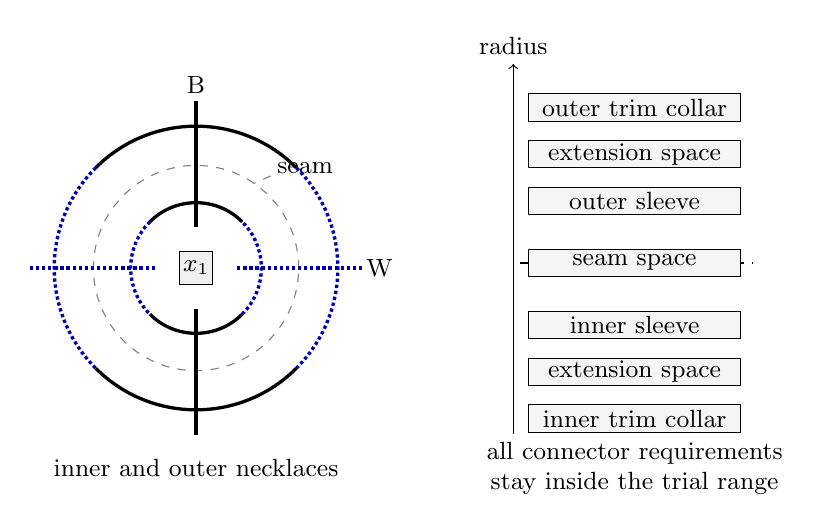
\begin{tikzpicture}[scale=0.79, every node/.style={font=\small}]
  \begin{scope}[xshift=-4.1cm]
    \draw[gray,dashed] (0,0) circle (1.65);
    \node[anchor=west] at (1.15,1.6) {seam};
    \draw[gray,dashed] (1.2,1.48)--(0.93,1.36);
    \foreach \r in {1.05,2.28} {
      \draw[very thick,black] (45:\r) arc (45:135:\r);
      \draw[very thick,blue!70!black,densely dotted] (135:\r) arc (135:225:\r);
      \draw[very thick,black] (225:\r) arc (225:315:\r);
      \draw[very thick,blue!70!black,densely dotted] (315:\r) arc (315:405:\r);
    }
    \draw[very thick,black] (90:0.66)--(90:2.68);
    \draw[very thick,black] (270:0.66)--(270:2.68);
    \draw[very thick,blue!70!black,densely dotted] (0:0.66)--(0:2.68);
    \draw[very thick,blue!70!black,densely dotted] (180:0.66)--(180:2.68);
    \draw[fill=gray!12] (-.27,-.27) rectangle (.27,.27);
    \node at (0,0) {$x_1$};
    \node at (0,2.94) {B};
    \node at (2.95,0) {W};
    \node[align=center] at (0,-3.22) {inner and outer necklaces};
  \end{scope}
  \begin{scope}[xshift=1cm,yshift=-2.42cm]
    \draw[->] (0,-.25)--(0,5.7) node[above] {radius};
    \draw[dashed] (.1,2.5)--(3.85,2.5);
    \foreach \y/\label in {0/inner trim collar,.75/extension space,1.5/inner sleeve,2.5/seam space,3.5/outer sleeve,4.25/extension space,5/outer trim collar} {
      \draw[fill=gray!8] (.25,\y-.22) rectangle (3.65,\y+.22);
      \node at (1.95,\y) {\label};
    }
    \node[align=center] at (1.95,-.8) {all connector requirements\\stay inside the trial range};
  \end{scope}
\end{tikzpicture}
\caption{The sewing construction, drawn schematically with round cycles.
Solid black and dotted blue denote the two colors.  Four ordered arms
carry the connection bit between necklaces across the deterministic seam.
The right-hand diagram gives the radial order of one trial; each displayed
space has fixed multiplicative width, with additional buffers between
supports.  Actual necklaces are site cycles, and the central forced region
is a square.}
\label{fig:sewing}
\end{figure}

For a fixed fair-bit environment, the connection bit at an inner necklace
is a monotone Boolean function $\phi$ of the bit imposed at the first
insertion.  This holds for both a single site and an entire square.  Thus
$\phi$ is constant or the identity.  At several times the same function
acts coordinatewise on the inserted history, because all other bits inside
the necklace are constant across time.

Fix the two environments and all histories at the other insertions.  For
now assume that every inactive-label crossing, if present, is unchanged
by the exchange; we establish this protection below.  Let $f_A(\mathbf h)$ be the
value of the exterior $F$ test when its outer necklace receives history
$\mathbf h$, and let $g_B(b)$ be the value of the exterior $G$ test when its outer
necklace receives bit $b$.  The necklace lemma makes these exterior
functions independent of which inside supplies the transmitted bit.
Write $a_A=\phi_A(1)-\phi_A(0)$ and
$a_B=\phi_B(1)-\phi_B(0)$, so $a_A,a_B\in\{0,1\}$.  Since both weights
are centered, the product of the signed responses before the exchange is
\begin{equation}
 \begin{aligned}
 &\left[\int f_A(\phi_A\circ\mathbf h)\,dw_1(\mathbf h)\right]
 \left[\int g_B(\phi_B(b))\,d\Delta(b)\right]
 \\
 &\qquad=a_Aa_B\left[\int f_A(\mathbf h)\,dw_1(\mathbf h)\right]
             \left[\int g_B(b)\,d\Delta(b)\right].
 \end{aligned}
 \label{eq:signed-bit-factorization}
\end{equation}
Here $\phi_A\circ\mathbf h$ means coordinatewise composition.  If a response
function is constant, centering annihilates its factor; otherwise it is
the identity.  Exchanging the insides exchanges $\phi_A$ and $\phi_B$,
while $f_A,g_B$ and their weights stay with the exterior tests.  The
right-hand side is unchanged.  This is a pointwise equality after the
signed history sums, not an equality between arbitrarily paired raw
histories.  Summing the other histories therefore preserves it.

\subsection{The adaptive exchange and relative error estimates}

Choose finitely many trial annuli with disjoint enlarged supports and a
seam in each.  All lie beyond both first-insertion scales.  Let $A_j$ be
the event that trial $j$ is the first successful trial in a fixed order,
and let $A_0$ be the event that none succeeds.  If $\mathcal T_j$ exchanges the
insides at trial $j$, define
\[
 \mathcal T(\omega^A,\omega^B)=
 \begin{cases}
 \mathcal T_j(\omega^A,\omega^B),&\text{on }A_j,\ j\ge1,\\
 (\omega^A,\omega^B),&\text{on }A_0.
 \end{cases}
\]
Each fixed exchange $\mathcal T_j$ preserves the product law: restrictions of
two independent marked Poisson processes to the inside are independent
and identically distributed, as are their fair bits.  On the lattice the
same observation applies to the bits.  The added nucleus is an annotation
that moves from the site environment to the other environment; no
Poisson intensity or Palm weight is changed.

The success status of trial $j$ is invariant under $\mathcal T_j$.  A trial farther
inside sees its two source environments exchanged wholesale, and a trial
farther outside is unchanged.  The success test is symmetric in its
sources, so every trial's status, and therefore $A_j$, is invariant under
$\mathcal T_j$.  The sets $A_0,A_1,\ldots$ partition the environment space; applying
a measure-preserving involution on each invariant piece proves that $\mathcal T$
is itself a measurable measure-preserving involution on the underlying
unannotated marked environments.  On its successful set it also exchanges
the site--square and square--site annotations.  On $A_0$ the annotations
stay in place, and we estimate that part separately.

We now estimate the error relative to the necessary four-arm probabilities.
First we remove failures of the microscopic screens.  An outer annulus
then protects the inactive replica, while many smaller annuli provide
trials for the active label.  The square radius $h$ will be taken below
all these trials only after their number and positions have been fixed.
Choose a fixed macroscopic probe radius $R$ sufficiently small for the
separations and tested boundaries.  Necessary probes at $x_i$, $i\ge2$,
have disjoint buffered supports from all the constructions at $x_1$;
they always contribute at most $C P_e$.  We therefore estimate only the
two environments at $x_1$.

Fix a large constant $M$.  By the outermost-failure estimate of
Lemma~\ref{lem:localization}, configurations contributing to either signed
product with an occupancy failure at a scale at least $M b_e$ in its site
probe have total probability at most
\begin{equation}
 \varepsilon(M)a_ea_{e,h},\qquad \varepsilon(M)\longrightarrow0.
 \label{eq:site-cutoff-error}
\end{equation}
For the square probe, failures above a constant multiple of $h$ contribute
$o_e(1)a_ea_{e,h}$ at each fixed $h$.  These estimates do not assume arms
on failed shells: group by the outermost failure, retain the necessary
probe beyond it with a disjoint buffer, and apply the power lower bound
and quasi-multiplicativity to sum the lost inner scales.

Outside these errors a necessary event $E$ consists of the occupancy
screens and four alternating active-label graph arms in both environments,
from scales comparable to $M b_e$ and $h$, respectively, to a scale
comparable to $R$.  Use deterministic graph-cycle cuts with room at the
ends.  These arms use the base fair bits: no inserted history reaches any
of their screened probe regions.  Although different crossing coordinates
may witness influence, the first insertion can influence only its active
label, so all these alternatives imply the same event $E$.  In particular
\begin{equation}
 \PP(E)\leq C(M,R)a_ea_{e,h}.
 \label{eq:necessary-probes-upper}
\end{equation}
The definition is made separately with the appropriate site and square
starting scales on the two sides of the comparison.  The event $E$ is
used only for upper bounds; the adaptive exchange is defined by its
symmetric success tests and does not require $E$ to be invariant.

Two ways of keeping these bounds relative will be used repeatedly.
First, let $J$ be a fixed positive-scale intermediate annulus, with
buffers, and let $H_J$ be a geometry event measurable in its enlargement
whose failure probability tends to zero.  Retain the necessary arm probes
strictly below and above that enlargement, in both environments.  These
probes are independent of its geometry.  Quasi-multiplicativity bounds
their product by $C(M,R)a_ea_{e,h}$ divided by the two fixed-ratio arm
costs omitted at $J$.  Those costs have positive mesh-uniform lower
bounds.  It follows that
\begin{equation}
 \PP(E\cap H_J^c)=o_e(1)a_ea_{e,h}.
 \label{eq:relative-typical-geometry}
\end{equation}
This also applies to geometry requirements in a sewn combination: a fixed
inside--outside combination has the ordinary Poisson law, and its local
geometry is still measurable in the two enlarged source annuli.  A finite
list of all such requirements is typical.  No typicality assertion is
being made at the microscopic scale $b_e$.

Second, choose $l_*>0$ much smaller than $R$ and put all trial annuli
strictly below $l_*$, with buffers.  When two replicas are used, impose the
following \emph{protection event} $H$: screening holds on an annulus from
constant multiples of $l_*$ to constant multiples of $R$, and in neither
source environment does the inactive label have four alternating arms
through that annulus.  It uses only sites above all the seams, hence is
invariant under every exchange.  If a tested crossing of the inactive
label changed after an exchange, the two configurations would agree on
this annulus and differ only on its inside.  The pivotal arm implication
would then give the forbidden four arms there.  The argument works for
every setting of the other histories, which are all outside the probe,
and includes changes of cells caused by the exchanged geometry.

For completeness, conditioning on the common geometry within this probe,
the two labels are independent.  If $p_e(\eta)$ is its quenched active
four-arm probability, the probability of four arms for both labels is
$\EE[p_e(\eta)^2]$, bounded by
$C A_e(l_*,R)^2$ by the second-moment arm estimate.  Retain the active
probe below it and the necessary probe in the other environment with
disjoint buffers.  Quasi-multiplicativity then gives
\begin{equation}
 \PP(E\cap H^c)
 \leq \bigl[C(M,R)A_e(l_*,R)+o_e(1)\bigr]a_ea_{e,h}.
 \label{eq:inactive-protection}
\end{equation}
Sum over which of the two source environments fails protection.  Fixed
radius changes are absorbed into the constant; mesh failures are covered
by \eqref{eq:relative-typical-geometry}.  The power upper bound makes the
bracket as small as desired by choosing $l_*/R$ small and then the mesh
small.  This extra arm factor is the reason common Poisson geometry for
the two replicas is compatible with the exchange argument.  With one
replica set $H$ equal to the entire probability space.

\subsection{Many annular trials}

It remains to show that $E$ almost always supplies a successful seam on
the relative scale $a_ea_{e,h}$.  Each trial has the radial layout in
Figure~\ref{fig:sewing}: an inner trim collar, an extension space, an inner
sleeve, a seam space, an outer sleeve, another extension space, and an
outer trim collar.  Every part has a fixed sufficiently large ratio.
Trim curves run through the middle of their collars; the deterministic
seam runs through the middle of its space.  The sleeve ratio is that of
Lemma~\ref{lem:necklace-sleeve}.  Include buffers between supports, and
choose all endpoint boxes and corridor routes from finite lists scaled
with the trial.  For any fixed number $n$, one can place $n$ such similar,
buffered trials below $l_*$ at fixed positive scales.  Subsequently take
$h$ below the innermost trial.

For trial $J$, let $T_J$ be the typical geometry event giving all its
screens, the quenched lower bounds for both sleeve constructions in both
environments, and all the
rectangle-crossing lower bounds for the corridor lists in every possible
sewn combination.  Screens in particular make each sleeve independent
of the source used on the far side of the seam.  Each sewn geometry has
the ordinary law, so a finite intersection supplies $T_J$.
Call $J$ \emph{disqualified}, an event denoted $B_J$, if $T_J$ fails or a
bad trim occurs at either of its two trim curves in either environment.
The bad trim test is the local close-approach event of
Lemma~\ref{lem:trim-arms}, including extra visits near the reserved
endpoint boxes.  Its paths are proper simple arms through a wider collar;
thus the two visits giving the test really yield four arms in a buffered
neighborhood, regardless of their color order.

For any $\rho>0$, the trim tolerance and the local geometry requirements
can be chosen so that, for every trial,
\begin{equation}
 \limsup_{e\downarrow0}
 \frac{\PP(E\cap B_J)}{a_ea_{e,h}}\leq\rho.
 \label{eq:trial-disqualification}
\end{equation}
Here and below $h$ is fixed below the trials.  For geometry failures this
is \eqref{eq:relative-typical-geometry}.  For a bad trim retain the
necessary parts of that environment's probe on both sides of its collar,
and the other environment's probe.  Their supports, including Poisson
buffers, avoid the bad test.  The absolute close-approach probability
multiplies their arm costs; deleting the fixed-ratio collar costs only a
fixed factor by quasi-multiplicativity.  Choose its tolerance to absorb
that factor.  This reasoning is uniform over scaled copies of the trial:
$\rho$ and the construction constants do not depend on $n$ or on a trial's
radius.  The mesh threshold may depend on the fixed finite collection.

Write $U_J$ for the symmetric successful seam event in trial $J$, and
$N=\bigcap_J U_J^c$ for failure of every trial.  The trials cannot be
treated as independent after restricting to the necessary long-arm event
$E$.  Instead, we compare failure of every trial with success of exactly
one specified trial.  The latter events are disjoint as that trial varies,
which will give the gain from the number of trials.

\begin{lemma}[One-trial comparison]
\label{lem:one-trial}
For the preceding fixed layouts and tolerances, there is $C_*<\infty$,
independent of the number of trials, their scales, and sufficiently small
mesh, such that
\begin{equation}
 \PP(E\cap N\cap B_J^c)
 \leq C_*\,
 \PP\left(E\cap U_J\cap\bigcap_{I\ne J}U_I^c\right)
 \label{eq:one-trial-comparison}
\end{equation}
for every trial $J$.
\end{lemma}

\begin{proof}
Condition first on all Poisson geometries, keeping only realizations in
$T_J$ and in the geometry part of $E$.  In each source environment retain
four arms from the inner beginning of its probe to the inner trim curve,
and four arms from its outer end down to the outer trim curve.  Stop at
first contact from the retained side, with the graph margins prescribed
above.  Since the trim is not bad, their endpoint boxes can be chosen from
a fixed finite list with matching cyclic order and the reserved avoidance
conditions.  For each choice let $\mathcal R$ be the event that such retained paths
exist, together with failure of all trials other than $J$.  Delete the
color part of disqualification, failure of trial $J$, and all arm
requirements between its two trims.  The events $\mathcal R$ for the finitely many
box and order choices cover the left-hand event of
\eqref{eq:one-trial-comparison}.  Their definition concerns existence of
retained paths; we do not reveal or condition on a selected path.

In the four sleeves, two in each source environment, impose the events
of Lemma~\ref{lem:necklace-sleeve}, with cardinal endpoint patches of
matching alternating colors.  Sleeve coordinates are disjoint from the
retained path coordinates and from the other trial supports.  Thus these
four events have joint conditional probability at least $c_0^4$, and
intersecting them with $\mathcal R$ costs at most that fixed factor.

We describe precisely the additional connector supports.  In each
extension space use disjoint polygonal tracks from the retained endpoint
boxes to the corresponding sleeve patches, first leaving the trim in its
normal direction and then respecting annular cyclic order.  At each end
start a track inside the box surrounded by the guarded lasso.  In the
seam space use four fixed separated tracks, of the same respective
colors for every inside--outside combination, and require rectangle-chain
connections in each of its four sewn geometries.  Every rectangle and
lasso used by a connector lies in these tracks or in a reserved endpoint
enlargement.  Include their cell stars in the supports.

Let $V_{\rm B}$ and $V_{\rm W}$ be, respectively, the original source-bit
coordinates used by black and white connector requirements, taking the
union over the four sewn combinations.  The positive widths between
opposite-color tracks and the mesh screens ensure
$V_{\rm B}\cap V_{\rm W}=\varnothing$; a source site cannot belong to two
opposite track supports, even if it is used in several sewn geometries.
On $V=V_{\rm B}\cup V_{\rm W}$ put the product order that favors black
on $V_{\rm B}$ and white on $V_{\rm W}$.  Every connector event is
increasing in this order.  Its conditional probability, with geometries
fixed, has a uniform positive lower bound from the crossing conditions
in $T_J$.  Harris' inequality therefore bounds the probability of all
connector events by a positive constant from below, since their number
is fixed.  These events depend only on the coordinates in $V$.

The retained-and-sleeve event has the same monotonicities on $V$.
For retained paths the only overlaps are their reserved, color-specific
endpoint enlargements.  For sleeves the only overlaps are their guarded
end patches; the five-arm exclusion giving the necklace lies strictly
in the core and uses no coordinate of $V$.  Requirements that paths avoid
other boxes are restrictions on allowed path locations, so favoring their
own colors preserves the existence of the required paths.  Failures of
other trials use no coordinate of $V$, or of these sleeves, because the
enlarged trial supports are disjoint.  They need not be monotone.

Now condition on all color coordinates outside $V$, apply Harris in $V$
to the retained-and-sleeve event and the intersection of the connector
events, and integrate back.  This costs another fixed positive factor.
All joining requirements are realized simultaneously, including those
in geometries that combine different sources.  Lassos ensure actual
connections to retained paths, while the reserved tracks ensure
disjointness, including between arms of the same color.  In the two
original environments the resulting arms complete $E$.  In all four
combinations they give $U_J$, with the common necklaces supplied by the
sleeves.  Other trials still fail.  Hence the probability for each retained
choice is at most a constant times the right-hand probability in
\eqref{eq:one-trial-comparison}.  Summing over the bounded finite choices
and then integrating the geometries proves the claim.
\end{proof}

Summing \eqref{eq:one-trial-comparison} over $n$ trials, its right-hand
events are pairwise disjoint.  On the left,
\[
 n\PP(E\cap N)
 \leq \sum_J\PP(E\cap N\cap B_J^c)+\sum_J\PP(E\cap B_J).
\]
Together with \eqref{eq:necessary-probes-upper} and
\eqref{eq:trial-disqualification}, this gives
\begin{equation}
 \limsup_{e\downarrow0}
 \frac{\PP(E\cap N)}{a_ea_{e,h}}
 \leq \rho+\frac{C_* C(M,R)}{n}.
 \label{eq:many-trials}
\end{equation}
The averaging over disqualifications, rather than a union bound over all
of them, is what leaves $\rho$ instead of $n\rho$.

\begin{proof}[Proof of Proposition~\ref{prop:replacement}]
Choose a desired relative error $z>0$.  First fix $M$ so that the cutoff
error in \eqref{eq:site-cutoff-error} is sufficiently small.  Next choose
$l_*/R$ so that \eqref{eq:inactive-protection} is sufficiently small.
Fix the sleeve and extension ratios, and the trim tolerances so that the
disqualification term $\rho$ is sufficiently small.  These choices fix
$C_*$.  Choose $n$ so large that $C_*C(M,R)/n$ is sufficiently small,
and place that many buffered trials below the protection annulus.
Only now take $h$ sufficiently small to lie below every trial; for each
such fixed $h$, let $e\downarrow0$.  All local constructions are therefore
at positive scales when their geometry conditions are imposed.

On configurations with a successful protected seam, the adaptive
measure-preserving involution and the signed identity following
Lemma~\ref{lem:necklace-bit} identify the two product integrals.
The remaining portions are bounded in total variation.  A nonzero
signed contribution has the necessary probes at every insertion point;
the independent probes at the other points contribute $C P_e$.  At the
first point the discarded portions are bounded by
\eqref{eq:site-cutoff-error}, \eqref{eq:inactive-protection}, and
\eqref{eq:many-trials}, together with the vanishing fixed-scale geometry
errors.  The weights contribute only their fixed total-variation bounds.
Thus the limsup of the ratio in
\eqref{eq:signed-relative-replacement} is at most $Cz$; since $z$ is
arbitrary, it is zero.

All constants are uniform on the fixed compact separated location range.
Local layouts are translated copies of the same finite lists.  In the
Poisson model Mecke points at other insertions lie outside their buffered
supports, and the screens make those annotations irrelevant there.  In
the triangular model translations are by lattice sites.  This proves
the stated uniformity and completes the comparison.
\end{proof}
